\usepackage{amsthm}

\newtheorem{theorem}{Theorem}[chapter]
\newtheorem{lemma}           [theorem] {Lemma}   
\newtheorem{folg}           [theorem] {Folgerung}   

\newtheorem{frage}       [theorem] {Frage}   
\newtheorem{question}       [theorem] {Question}   
\newtheorem{aufgabe}       [theorem] {Aufgabe}   
\newtheorem{exercise}       [theorem] {Exercise}  

\newtheorem{proposition}     [theorem] {Proposition}  
\newtheorem{satz}     [theorem] {Satz}  
\newtheorem{fact}{Fact}
\newtheorem{definition}      [theorem] {Definition} 

\theoremstyle{definition} 
\newtheorem{bemerkung}     [theorem] {Bemerkung}  
\newtheorem{beispiel}       [theorem] {Beispiel}  
\newtheorem{example}       [theorem] {Example}  
\newtheorem*{example*} {Example}  
\newtheorem{notation}       [theorem] {Notation}  
\newtheorem*{Faust}[theorem]{Rule of Thumb}
\newtheorem*{Boxx}[theorem]{Concept}

Here we consider derivatives of derivatives (of derivatives ...) and discuss consequences for the search for local extrema of functions.

\begin{Definition}{}
If the derivative of a~function is differentiable, we call $(f')'$ the \emph{second derivative}. The \emph{$n$-th derivative of a~function} is inductively defined as the derivative of the $n-1$-th derivative.\\
For the second derivative at $x_0$, we write
$f''(x_0)$ or $\frac{d^2}{dx^2}f(x_0)$. The $n$-th derivative is denoted by
$f^{(n)}(x_0)$ or $\frac{d^n}{dx^n}f(x_0)$.\\
    We call a~function $f:I\to\mathbb{R}$ \emph{$n$-times differentiable} if $f^{(n)}(x)$ exists for all $x\in I$.\\
    Furthermore we call a~function $f:I\to\mathbb{R}$ \emph{$n$-times continuously differentiable} if $f^{(n)}:I\to\mathbb{R}$ exists and is continuous.\\
\end{Definition}

\begin{Theorem}{}\label{th:localextr}
    Let $I:=[a,b]$ and $f:I\to\mathbb{R}$ be differentiable. Furthermore let $x_0\in I$ such that $f'(x_0)=0$ and $f'$ is differentiable in $x_0$. Then
\begin{enumerate}
 \item if $f''(x_0)>0$, then $f$ has a local minimum in $x_0$;
 \item if $f''(x_0)<0$, then $f$ has a local maximum in $x_0$.
\end{enumerate}
\end{Theorem}
{\em Proof:} We only show the case $f''(x_0)>0$ (the opposite case is analogous). By definition, we have
\[f''(x_0)=\lim_{x\to x_0}\frac{f'(x)-f'(x_0)}{x-x_0}>0.\]
Since $f'$ is continuous in $x_0$, we have that there exists some $\varepsilon>0$ such that for all $x\in I\backslash\{x_0\}$ 
with $|x-x_0|<\varepsilon$ holds
\[\frac{f'(x)-f'(x_0)}{x-x_0}>0.\]
Since $f'(x_0)=0$, we have that
\[
\begin{aligned}
 f'(x)<0&\quad\text{for all }x\in(x_0-\varepsilon,x_0),\\
 f'(x)>0&\quad\text{for all }x\in(x_0,x_0+\varepsilon).
\end{aligned}
\]
Therefore, $f$ is monotonically decreasing in $(x_0-\varepsilon,x_0)$ and monotonically increasing in 
$(x_0,x_0+\varepsilon)$. 
Therefore, $f$ has a local minimum in $x_0$.\hfill$\Box$
\begin{Remark}{}
 Note that in the case $f''(x_0)=0$, we cannot make a~decision whether $f$ has a~local extremum there. 
 For instance, consider the three functions $f_1(x)=x^3$, $f_2(x)=x^4$ and $f_3(x)=-x^4$. We have $f_1'(0)=f_2'(0)=f_3'(0)=0$ and, 
 furthermore, $f_1''(0)=f_2''(0)=f_3''(0)=0$. However, $f_1$ has no local extremum in $0$, $f_2$ has a local minimum in $0$ and $f_3$ 
 has a~local maximum in $0$.
\end{Remark}

\begin{example}
\begin{enumerate}
 \item Consider the rational function
\[f(x)=\frac{x(x+5)}{x-4}=x+9+\frac{36}{x-4}.\]
It can be easily seen that $f$ has a first order pole at $x_0=4$.\\
The first two derivatives of $f$ are given by
\[f'(x)=\frac{x^2-8x-20}{(x-4)^2}=\frac{(x+2)(x-10)}{(x-4)^2},\qquad f''(x)=\frac{72}{(x-4)^3}.\]
The zeros of $f$ are given by $x_1=0$ and $x_2=-5$.\\% Since $f'(0)=-\frac54<0$, the function is monotonically decreasing in a~neighborhood of $x_1=0$.
%Since $f'(-5)=45>0$, the function is monotonically increasing in a~neighborhood of $x_2=-5$.\\
Now we determine the set of local extrema: We have that $f'(x)=0$ is only fulfilled for $x_3=-2$ and $x_4=10$. In this case, we have $f''(x_3)=-\frac13<0$ and $f''(x_4)=\frac13>0$. As a~consequence, $f$ has a~local maximum in $x_3=-2$ and a~local minimum in $x_4=10$. We further have
\begin{itemize}
 \item[a)] $x\in(-\infty,-2)~\Rightarrow f'(x)>0$, i.e., $f$ is strictly monotonically increasing in 
 $(-\infty,-2)$;
 \item[b)] $x\in(-2,4)~\Rightarrow f'(x)<0$, i.e., $f$ is strictly monotonically decreasing in $(-2,4)$;
 \item[c)] $x\in(4,10)~\Rightarrow f'(x)<0$, i.e., $f$ is strictly monotonically decreasing in $(4,10)$;
 \item[d)] $x\in(10,\infty)~\Rightarrow f'(x)>0$, i.e., $f$ is strictly monotonically increasing in 
 $(10,\infty)$.
\end{itemize}
\item $f(x)=\sin(x)$. The zeros are given by
    \[\{0,\pi,-\pi,2\pi,-2\pi,3\pi,-3\pi,\ldots\}=\{n\pi\;|\;n\in\mathbb{Z}\}.\]
The first two derivatives are given by $f'(x)=\cos(x)$, $f''(x)=-\sin(x)$. The zeros of $f'$ are given by
        \[\left\{\frac\pi2,-\frac\pi2,\frac{3\pi}2,-\frac{3\pi}2,\frac{5\pi}2,\frac{5\pi}2,\ldots\right\}=\left\{\frac{2n+1}2\pi\;|\;n\in\mathbb{Z}\right\}.\]
For $x_n=\frac{2n+1}2\pi$, we have $f''(x_n)=-\sin(\frac{2n+1}2\pi)=(-1)^{n+1}$. As a~consequence, $\sin$ has a~local maximum in $x_n=\frac{2n+1}2\pi$ if $n$ is even and a~local minimum in $x_n=\frac{2n+1}2\pi$ if $n$ is odd.
\end{enumerate}
\end{example}

\begin{Definition}[Convexity/Concavity] \label{def:convexity}
    A function $f:[a,b]\rightarrow \mathbb{R}$, $a,b\in\mathbb{R}$, $a<b$, is called \emph{convex}, if for all $x_1<x<x_2$ in $[a,b]$ holds
    \begin{equation}\label{eq:convex} 
      f(x) \leq \frac{f(x_2)-f(x_1)}{x_2-x_1}\cdot(x-x_1)+f(x_1)\ .      
    \end{equation}
    It is called \emph{concave}, if for all $x_1<x<x_2$ in $[a,b]$ holds
    \begin{equation}\label{eq:concave} 
      f(x)\geq \frac{f(x_2)-f(x_1)}{x_2-x_1}\cdot(x-x_1)+f(x_1)\ .
    \end{equation}
    If the inequalities in (\ref{eq:convex}) or (\ref{eq:concave}) are strict then $f$ is called \emph{strictly convex/concave}.
    
Geometrically this means that the graph of a convex (concave) function $f:[a,b]\rightarrow \mathbb{R}$ restricted to any subinterval 
$[x_1,x_2]$ of $[a,b]$ lies 
below (above) the secant $$s(x):=\frac{f(x_2)-f(x_1)}{x_2-x_1}\cdot(x-x_1)+f(x_1) \ .$$
\end{Definition}

% %\begin{minipage}[t]{120mm}
% \begin{figure}[htp]
% \begin{center}
% \includegraphics[width=0.4\textwidth,angle=0]{pics/fconvex.eps} 
% \includegraphics[width=0.4\textwidth,angle=0]{pics/fconcave.eps} 
% \caption{convex and concave graphs}
% \label{fig:convex}
% \end{center}
% \end{figure}
% %\end{minipage}

\begin{Theorem}{} \label{th:convconc}
    Let $f:[a,b]\rightarrow \mathbb{R}$, $a,b\in\mathbb{R}$, $a<b$, be 2-times differentiable. 
  \begin{enumerate}
   \item[a)]   If $f''(x)\geq 0$ for all $x\in~(a,b)$~, then $f$ is convex.
   \item[b)]   If $f''(x)>0$ for all $x\in~(a,b)$~, then $f$ is strictly convex.
   \item[c)]   If $f''(x)\leq 0$ for all $x\in~(a,b)$~, then $f$ is concave.
   \item[d)]   If $f''(x)<0$ for all $x\in~(a,b)$~, then $f$ is strictly concave.
  \end{enumerate}
\end{Theorem}

{\em Proof:} We only prove a). The other results follow analogously. 
  Let $x_1<x<x_2$ in $[a,b]$. Since $f''\geq 0$ we know that $f'$ is monotonically increasing.
  By the intermediate value theorem there are $\xi_1\in~(x_1,x)$ and $\xi_2\in~(x,x_2)$ such that
  \begin{eqnarray*}
    \frac{f(x)-f(x_1)}{x-x_1} &=& f'(\xi_1) \leq f'(\xi_2) = \frac{f(x_2)-f(x)}{x_2-x} \ .
  \end{eqnarray*}

  This implies
  \begin{eqnarray*}
    && (f(x)-f(x_1))(x_2-x) \leq (f(x_2)-f(x))(x-x_1) \\ \\
    &\Leftrightarrow& f(x)(x_2-x_1) \leq (f(x_2)-f(x_1))(x-x_1)+f(x_1)(x_2-x_1) \\
    &\Leftrightarrow& f(x) \leq \frac{f(x_2)-f(x_1)}{x_2-x_1}(x-x_1)+f(x_1)\ .   
  \end{eqnarray*}
\hfill$\Box$

\begin{Definition}{Inflection point}
    Let $f:[a,b]\rightarrow \mathbb{R}$ be a function. We say that $x_0\in ~(a,b)$ is an \emph{inflection point} of $f$ if there is an $\varepsilon>0$ with 
    $[x_0-\varepsilon,x_0+\varepsilon]\subset[a,b]$ such that one of the following two statements holds true:
    \begin{enumerate}
     \item[a)] $f$ is convex on $[x_0-\varepsilon,x_0]$ and concave on $[x_0,x_0+\varepsilon]$.
     \item[b)] $f$ is concave on $[x_0-\varepsilon,x_0]$ and convex on $[x_0,x_0+\varepsilon]$.
    \end{enumerate}
\end{Definition}

\begin{Theorem}{}
    Let $f:[a,b]\rightarrow \mathbb{R}$ be 3-times continuously differentiable and $x_0\in~(a,b)$. 
  \begin{enumerate}
   \item[a)] If $x_0$ is an inflection point, then $f''(x_0)=0$.
   \item[b)] If $f''(x_0)=0$ and $f'''(x_0)\neq 0$, then $x_0$ is an inflection point.  
  \end{enumerate}
\end{Theorem}

{\em Proof:} 
a) follows from Theorem \ref{th:convconc} and continuity of $f''$.

b) If $f''(x_0)=0$ and $f'''(x_0)\neq 0$, then by continuity of $f'''$ there is an $\varepsilon>0$ with 
   $[x_0-\varepsilon,x_0+\varepsilon]\subset[a,b]$ such that $f'''$ does not have a zero on $[x_0-\varepsilon,x_0+\varepsilon]$.
   This implies that $f''$ is strictly monotonic on $[x_0-\varepsilon,x_0+\varepsilon]$. Thus either
   \begin{enumerate}
    \item[i)] $f''>0$ on $[x_0-\varepsilon,x_0]$ and  $f''< 0$ on $[x_0,x_0+\varepsilon]$ or
    \item[ii)] $f''< 0$ on $[x_0-\varepsilon,x_0]$ and  $f''> 0$ on $[x_0,x_0+\varepsilon]$
   \end{enumerate}
   holds true.
   In case i), $f$ is convex on $[x_0-\varepsilon,x_0]$ and concave on $[x_0,x_0+\varepsilon]$ and 
   in case ii) the reversed behavior is given.
   Therefore $x_0$ is an inflection point.
\hfill$\Box$
 \\ \\
The aim of a so-called \emph{curve discussion} of a function $f:D\rightarrow \mathbb{R}$, $D\subset \mathbb{R}$, is to determine its qualitative and 
quantitative behaviour. We give a short list of things that have to be investigated/determined:

\begin{enumerate}
 \item[1.] Domain of definition $D$
 \item[2.] Symmetries
    \begin{enumerate}
    \item[a)] $f$ is symmetrical with respect to the $y$-axis if $f(x)=f(-x)$ for all $x$ in the domain of definition.
              In this case $f$ is called an even function.
    \item[b)] $f$ is point-symmetrical with respect to the origin if $f(-x)=-f(x)$ for all  $x$ in the domain of definition.
              In this case $f$ is called an odd function.
    \end{enumerate}
  \item[3.] Poles
  \item[4.] Behaviour for $x\longrightarrow \pm\infty$, asymptotes
      
      A straight line $g(x)=ax+b$, $a,b\in\mathbb{R}$, is called an asymptote of $f$ for $x\rightarrow\pm\infty$ 
            if $\lim_{x\rightarrow\pm\infty}(f(x)-(ax+b)) = 0$. In this case the coefficients $a,b$ can be 
            successively determined by
	    \begin{eqnarray*}
	     a &=& \lim_{x\rightarrow\pm\infty}\frac{f(x)}{x}\ , \\
	     b &=& \lim_{x\rightarrow\pm\infty}(f(x)-ax) \ .
	    \end{eqnarray*}
  \item[5.] Zeros
  \item[6.] Extrema, monotonicity behaviour
  \item[7.] Inflection points, convexity/concavity behaviour
  \item[8.] Function graph
\end{enumerate}
 
 
 \whiteskip

\begin{example}
  We want to give a complete curve discussion for the rational function 
  $$f(x)=\frac{2x^2+3x-4}{x^2} \ .$$
\begin{enumerate}
    \item[1.] Domain of definition: $D=\mathbb{R}\backslash\{0\}$
 \item[2.] Symmetries: $f$ is neither an even nor an odd function.
 \item[3.] Poles: $x_0=0$ is a pole of order $2$, $\lim_{x\nearrow 0}f(x)=-\infty=\lim_{x\searrow 0}f(x)$
 \item[4.] Behaviour for $x\longrightarrow \pm\infty$, asymptotes:      
	     $\lim_{x\rightarrow\pm\infty}\frac{f(x)}{x} = 0$,
	     $\lim_{x\rightarrow\pm\infty} f(x) =2$.
            Thus the horizontal line at $y=2$ is an asymptote of $f$ for $x\longrightarrow \infty$  and also for $x\longrightarrow -\infty$.
 \item[5.] Zeros: $f(x)=0 \ \Leftrightarrow \ 2x^2+3x-4=0 \ \Leftrightarrow \  x=x_{1,2}=\frac{1}{4}(-3\pm\sqrt{41})$\\
            $x_1\approx-2.35$,  $x_2\approx 0.85$	    
 \item[6.] Extrema, monotonicity behaviour:
	    
            $f'(x)=\frac{-3x+8}{x^3}=0 \ \Leftrightarrow \ x=x_3= \frac{8}{3}$, $y_3:=f(x_3)\approx 2.56$

	    $f''(x)=\frac{6x-24}{x^4}$  
              
            $f''(x_3)<0 \ \Rightarrow \ $ $f$ has a local maximum at $x_3$.    

        \[ f'(x) \quad \left\{
 	\begin{array}{lll}
	  <0 &, \frac{8}{3} <x <\infty & \text{, strictly monotonically decreasing} \\
	  >0 &, 0<x<\frac{8}{3}        & \text{, strictly monotonically increasing} \\
	  <0 &, -\infty<x<0            & \text{, strictly monotonically decreasing} 
 	\end{array}
         \right.
         \]

 \item[7.] Inflection points, convexity/concavity behaviour:
      
      $f''(x)=0 \ \Leftrightarrow \  x=x_4=4$, $y_4=f(x_4)=\frac{5}{2}$

      $f'''=\frac{96-18x}{x^5}$ 

      $f'''(x_4)>0 \ \Rightarrow \ $ $x_4$ is an inflection point.


        \[ f''(x) \quad \left\{
 	\begin{array}{lll}
	  >0 &, 4 <x <\infty 	 	& \text{, strictly convex} \\
	  <0 &, 0<x<4         & \text{, strictly concave} \\
	  <0 &, -\infty<x<0             & \text{, strictly concave} 
 	\end{array}
         \right.
         \]
%   \item[8.] Function graph
%  \begin{figure}[htp]
%  \begin{center}
%  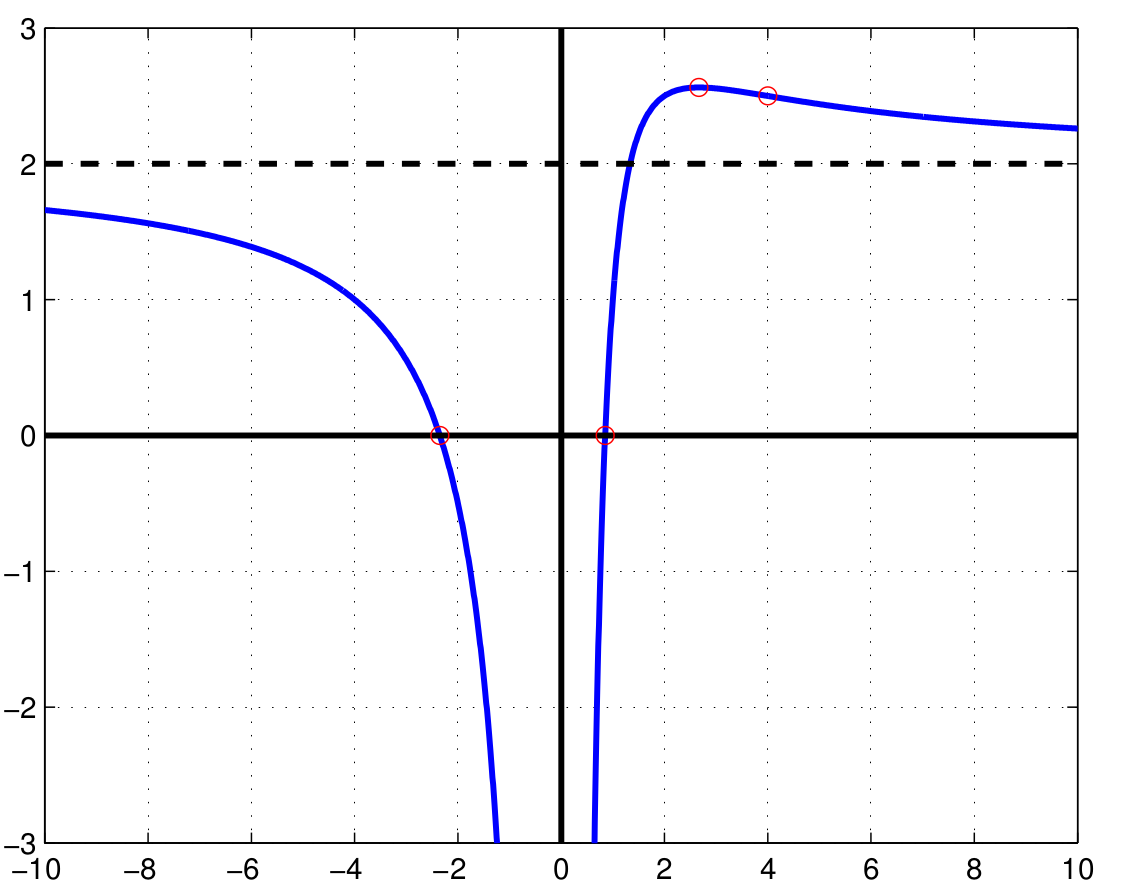
\includegraphics[width=0.8\textwidth,angle=0]{pics/curvedisc.eps} 
%  %\caption{}
%  \label{fig:convex}
%  \end{center}
%  \end{figure}
\end{enumerate}
\end{example}

